\documentclass{article}
\usepackage[utf8]{inputenc}
\usepackage{tikz}
\usepackage{circuitikz}
\usepackage{geometry}
\geometry{margin=1in}
\usepackage{listings}
\usepackage{xcolor}
\geometry{margin=1in}
\title{IR Sensor Documentation - Raspberry Pi 5 Integration}
\author{El Mehdi Adnani Kadmiri}
\date{July 17, 2025}

\lstset{
	basicstyle=\ttfamily\small,
	keywordstyle=\color{blue},
	commentstyle=\color{gray},
	stringstyle=\color{teal},
	breaklines=true,
	frame=single,
	postbreak=\mbox{\textcolor{red}{$\hookrightarrow$}\space}
}

\begin{document}
	
	\maketitle
	
	\section{Description}
	An Infrared (IR) sensor is an electronic device that emits infrared light and detects its reflection to sense the presence of objects or surface types (light/dark). It is commonly used in two ways:
	\begin{itemize}
		\item \textbf{Line Detection:} Follows black or white tracks, used in robotic pathfinding.
		\item \textbf{Proximity Detection:} Detects nearby obstacles or objects without contact.
	\end{itemize}
	
	\section{Applications}
	\begin{itemize}
		\item Line-following robots
		\item Proximity and obstacle avoidance systems
		\item Automation and safety in industrial systems
	\end{itemize}
	
	\section{Working Principle}
	IR sensors use an IR LED to emit light, and a photodiode or phototransistor to detect reflections. Light-colored surfaces reflect more IR light, producing a high signal, while dark surfaces absorb IR light, producing a low signal. The sensor typically outputs a \textbf{digital HIGH or LOW signal}.
	
	\section{Wiring Diagram}
	\begin{center}
		\begin{tabular}{|c|c|c|}
			\hline
			\textbf{IR Sensor Pin} & \textbf{Raspberry Pi Pin} & \textbf{Function} \\
			\hline
			VCC & 3.3V or 5V & Power \\
			GND & GND & Ground \\
			OUT & GPIO17 (or any input) & Digital Output \\
			\hline
		\end{tabular}
	\end{center}
	
		\begin{center}
		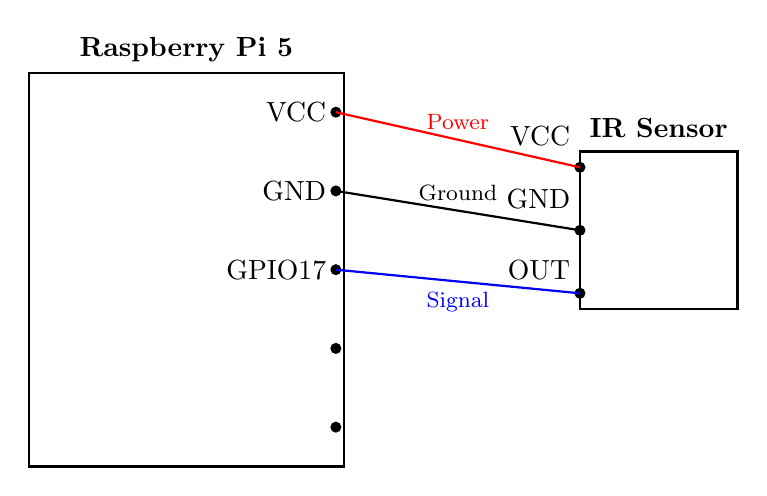
\begin{tikzpicture}
			
			% Raspberry Pi rectangle
			\draw[thick] (0,0) rectangle (4,5);
			\node at (2,5.3) {\textbf{Raspberry Pi 5}};
			\node[anchor=east] at (3.9,4.5) {VCC};
			\node[anchor=east] at (3.9,3.5) {GND};
			\node[anchor=east] at (3.9,2.5) {GPIO17};
			% GPIO pins
			
			\fill (3.9,4.5) circle (2pt); % 3.3V
			\fill (3.9,3.5) circle (2pt); % GND
			\fill (3.9,2.5) circle (2pt);
			\fill (3.9,1.5) circle (2pt);
			\fill (3.9,0.5) circle (2pt);
			 
			 
			
			% IR Sensor rectangle
			\draw[thick] (7,2) rectangle (9,4);
			\node at (8,4.3) {\textbf{IR Sensor}};
			% Sensor pins
			\node[anchor=east] at (7,4.2) {VCC};
			\node[anchor=east] at (7,3.4) {GND};
			\node[anchor=east] at (7,2.5) {OUT};
			% Dots for sensor pins
			\fill (7,3.8) circle (2pt); % VCC
			\fill (7,3.0) circle (2pt); % GND
			\fill (7,2.2) circle (2pt); % OUT
			
			% Connecting lines
			\draw[red, thick] (3.9,4.5) -- (7,3.8) node[midway, above] {\footnotesize Power};
			\draw[black, thick] (3.9,3.5) -- (7,3.0) node[midway, above] {\footnotesize Ground};
			\draw[blue, thick] (3.9,2.5) -- (7,2.2) node[midway, below] {\footnotesize Signal};
			
		\end{tikzpicture}
		\end{center}
		
	
	\section{Libraries Used}
	\subsection*{Python: RPi.GPIO}
	This library allows GPIO pin configuration and digital input/output operations.
	\begin{itemize}
		\item Setup with: \texttt{import RPi.GPIO as GPIO}
		\item Set pin mode: \texttt{GPIO.setmode(GPIO.BCM)}
		\item Read value: \texttt{GPIO.input(17)}
	\end{itemize}
	
	\subsection*{C: wiringPi}
	\texttt{wiringPi} is a C library for Pi GPIO control.
	\begin{itemize}
		\item Setup: \texttt{wiringPiSetup()}
		\item Set pin mode: \texttt{pinMode(0, INPUT)}
		\item Read value: \texttt{digitalRead(0)}
	\end{itemize}
	
	\section{Python Example}
	\begin{lstlisting}[language=Python]
		import RPi.GPIO as GPIO
		import time
		
		SENSOR_PIN = 17
		
		GPIO.setmode(GPIO.BCM)
		GPIO.setup(SENSOR_PIN, GPIO.IN)
		
		try:
		while True:
		if GPIO.input(SENSOR_PIN):
		print("No obstacle detected")
		else:
		print("Obstacle detected")
		time.sleep(0.5)
		except KeyboardInterrupt:
		GPIO.cleanup()
	\end{lstlisting}
	
	\section{C Example}
	\begin{lstlisting}[language=C]
		#include <wiringPi.h>
		#include <stdio.h>
		
		#define SENSOR_PIN 0 // wiringPi pin 0 = BCM 17
		
		int main(void) {
			wiringPiSetup();
			pinMode(SENSOR_PIN, INPUT);
			
			while (1) {
				int value = digitalRead(SENSOR_PIN);
				if (value == HIGH)
				printf("No obstacle detected\n");
				else
				printf("Obstacle detected\n");
				delay(500);
			}
			
			return 0;
		}
	\end{lstlisting}
	
	\section{Conclusion}
	The IR sensor is a simple, responsive, and low-cost component ideal for basic object detection tasks. It provides an easy introduction to GPIO interaction on the Raspberry Pi using both C and Python.
	
\end{document}
